\chapter{基于奇异关联子的弦网模型基态构建}

\tikzset{x=1em, y=1em, node font=\footnotesize}
\newcommand{\Vertex}[3]{
  \begin{tikzpicture}[baseline=0, thick]
    \draw (0,0) -- (90:1)  node [above] {$#1$}
          (0,0) -- (210:1) node [left]  {$#2$}
          (0,0) -- (330:1) node [right] {$#3$};
  \end{tikzpicture}
}

\section{弦网模型基态的张量网络表示}

接下来我们来给出弦网模型的基态表示\cite{gu2009tensor2,buerschaper2009explicit}。由于弦网模型的 Hamilton 量
\begin{equation}
  H = -\sum_v A_v - \sum_p B_p
\end{equation}
是严格可解的,即可以表示成一系列相互对易的投影算符之和,因而它的基态可以通过这些投影算符的本征子空间给出。式中,电荷算符 $A_v$ 指定了每个顶点处的融合规则:
\begin{equation}
  A_v \Biggl| \Vertex ijk \Biggr\rangle = \delta_{ijk} \Biggl| \Vertex ijk \Biggr\rangle, \quad
  \delta_{ijk} = \begin{cases}
    1, & \text{if $(i,j,k)$ is allowed to fuse;} \\
    0, & \text{otherwise;}
  \end{cases}
\end{equation}
磁通量算符 $B_p$ 定义为
\begin{equation}
  B_p = \sum_{s=0}^N \frac{d_s}{D} B_p^s,
\end{equation}
其中
\begin{equation}
  D = \sum_s d_s^2
\end{equation}
是总量子维数,而 $B_p^s$ 则可以图形化地视为能在方块 $p$ 处生成一个孤立环路的算符[具体定义见 \eqref{eq:string-net-bp} 式]。

于是弦网模型的基态波函数 $\ket{\psi_0}$ 可以通过在真空态 $\ket{\varnothing}$ 上作用全部的 $B_p$ 算符得到。如上所言,每个 $B_p$ 算符都是一个方块内部由对象 $R$ 构成的环路,而
\begin{equation}
  \tikz [baseline=0, very thick, draw=MaterialRed]
    \draw (0,-1) node [left] {$R$} -- (0,1.5);
  \enspace = \sum_i \frac{d_i}{D}
  \tikz [baseline=0, thick]
    \draw (0,-1) node [left] {$i$} -- (0,1.5);
\end{equation}
则是任意子按量子维数的加权叠加。因此有
\begin{equation}
  \newcommand{\VirutalLoop}{
    \draw [thick, dotted]
      (0,0) -- ++(330:1) -- ++( 30:1) -- ++( 90:1) -- ++(150:1) -- ++(210:1)
      (0,0) -- ++( 90:1) -- ++(150:1) -- ++(210:1) -- ++(270:1) -- ++(330:1)
      (0,0) -- ++(210:1) -- ++(270:1) -- ++(330:1) -- ++( 30:1) -- ++( 90:1);
  }
  \ket{\psi_0} = \prod_p B_p \ket{\varnothing} = \prod_p B_p \,
  \Biggl| \,
  \tikz [baseline=-0.3em] \VirutalLoop;
  \, \Biggr\rangle = \Biggl| \,
  \begin{tikzpicture}[baseline=-0.3em]
    \VirutalLoop;
    \draw [very thick, draw=MaterialRed]
      ( 30:1) circle [radius=0.55]
      (150:1) circle [radius=0.55]
      (270:1) circle [radius=0.55];
  \end{tikzpicture}
  \, \Biggr\rangle.
\end{equation}

为了给出 $\ket{\psi_0}$ 一种\emph{对称化}的张量网络表示,我们必须从一开始就同等对待六边形的每个边以保持对称性。需要指出的是,文献 \parencite{buerschaper2009explicit} 中通过引入奇偶子格点来构造张量网络的手段不能很好地保留旋转对称性。这里,我们需将权重(量子维数)$d_i$ 平均分配到 $R$ 环路的六个边上,使得它们在互相连接时也有良好定义:
\begin{equation}
  \newcommand{\VirutalHexagon}{
    \draw [thick, dotted]
      (30:1.2) -- (90:1.2) -- (150:1.2) -- (210:1.2) -- (270:1.2) -- (330:1.2) -- cycle;
  }
  \begin{aligned}
    % 1 segment
    \begin{tikzpicture}[baseline=-0.2em]
      \VirutalHexagon;
      \draw [very thick, draw=MaterialRed] (-30:0.8) -- (30:0.8);
    \end{tikzpicture}
    \enspace &= \sum_i \biggl( \frac{d_i}{D} \biggr)^{1/6} \enspace
    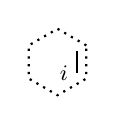
\begin{tikzpicture}[baseline=-0.2em]
      \VirutalHexagon;
      \draw [thick] (-30:0.8) node [left] {$i$} -- (30:0.8);
    \end{tikzpicture} \, , \\
    % 2 segments
    \begin{tikzpicture}[baseline=-0.2em]
      \VirutalHexagon;
      \draw [very thick, draw=MaterialRed] (-30:0.8) -- (30:0.8) -- (90:0.8);
    \end{tikzpicture}
    \enspace &= \sum_i \biggl( \frac{d_i}{D} \biggr)^{1/3} \enspace
    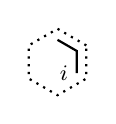
\begin{tikzpicture}[baseline=-0.2em]
      \VirutalHexagon;
      \draw [thick] (-30:0.8) node [left] {$i$} -- (30:0.8) -- (90:0.8);
    \end{tikzpicture} \, , \\
    % Loop
    \begin{tikzpicture}[baseline=-0.2em]
      \VirutalHexagon;
      \draw [very thick, draw=MaterialRed] (0,0) circle [radius=0.7];
    \end{tikzpicture}
    \enspace &= \sum_i \frac{d_i}{D} \enspace
    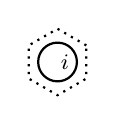
\begin{tikzpicture}[baseline=-0.2em]
      \VirutalHexagon;
      \draw [thick] (0,0) circle [radius=0.7] node [right=-0.2em] {$i$};
    \end{tikzpicture} \, .
  \end{aligned}
\end{equation}
对于邻接的六边形,我们可以在两个相邻的 $R$ 环路间执行 $F$ 移动:
\begin{align}
  \begin{tikzpicture}[baseline=-0.2em]
    \draw [thick, dotted]
      (30:1.2) -- (90:1.2) -- (150:1.2) -- (210:1.2) -- (270:1.2) -- (330:1.2)
      -- ++(-30:1.2) -- ++(30:1.2) -- ++(90:1.2) -- ++(150:1.2) -- ++(210:1.2) -- ++(270:1.2);
    \draw [very thick, draw=MaterialRed]
      (-30:0.8) -- ++(90:0.8)
      (-30:1.2) ++ (30:0.4) -- ++(90:0.8);
  \end{tikzpicture}
  \enspace &= \sum_{i,j} \biggl( \frac{d_i d_j}{D^2} \biggr)^{1/6} \enspace
  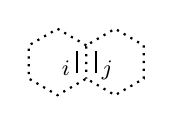
\begin{tikzpicture}[baseline=-0.2em]
    \draw [thick, dotted]
      (30:1.2) -- (90:1.2) -- (150:1.2) -- (210:1.2) -- (270:1.2) -- (330:1.2)
      -- ++(-30:1.2) -- ++(30:1.2) -- ++(90:1.2) -- ++(150:1.2) -- ++(210:1.2) -- ++(270:1.2);
    \draw [thick]
      (-30:0.8) -- ++(90:0.8)
      (-30:1.2) ++ (30:1.2-0.8) -- ++(90:0.8)
      (0.3,-0.5) node [anchor=base] {$i$}
      (1.8,-0.5) node [anchor=base] {$j$};
  \end{tikzpicture}
  \notag \\
  &= \sum_{i,j} \biggl( \frac{d_i d_j}{D^2} \biggr)^{1/6} \sum_k \sqrt{\frac{d_k}{d_i d_j}} \enspace
  \tikz [thick, baseline=-0.2em]
    \draw (90:0.6) -- +(150:1.2) node [above] {$i$} -- +(0,0) -- +(30:1.2) node [above] {$j$}
          +(0,0) -- (-90:0.6)
          +(0,0) -- +(-150:1.2) node [below] {$i$} -- +(0,0) -- +(-30:1.2) node [below] {$j$}
          (0,0) node [right] {$k$};
  \notag \\
  &= \sum_{i,j,k} \bigl( D d_i d_j \bigr)^{-1/6} d_k^{1/4} \enspace
  \begin{tikzpicture}[thick, baseline=-0.5em]
    \draw [draw=MaterialIndigo]
      (0,0) -- (270:1.2) node [below] {$k$};
    \draw [draw=MaterialPurple]
      (150:1.2) node [above=0.4, anchor=base] {$i$} -- (0,0) --
      ( 30:1.2) node [above=0.4, anchor=base] {$j$};
  \end{tikzpicture}
  \cdot \bigl( D d_i d_j \bigr)^{-1/6} d_k^{1/4} \enspace
  \begin{tikzpicture}[thick, baseline=-0.2em]
    \draw [draw=MaterialIndigo]
      (0,0) -- ( 90:1.2) node [above] {$k$};
    \draw [draw=MaterialPurple]
      (210:1.2) node [below] {$i$} -- (0,0) --
      (-30:1.2) node [below] {$j$};
  \end{tikzpicture} \, .
\end{align}
此处蓝线和紫线分别代表 $d^{-1/6}$ 和 $d^{1/4}$ 的因子。于是 $\ket{\psi_0}$ 中的每个顶点可以写成
\begin{align}
  \text{[TODO]}
\end{align}

% TODO:
在对所有的 $R$ 环路执行 $F$ 移动之后,$\ket{\psi_0}$ 现在可以表示为
\begin{equation}
  \ket{\psi_0} = ...
\end{equation}
它可以通过对位于顶点处的局域构建块进行缩并得到,并且可以用任意子基表示为
\begin{equation}
  ...
\end{equation}
这样我们就获得了六边形网格中三角形张量的对称形式:
\begin{align}
  \text{[diagram]}
  &= (d_i d_j d_k)^{-\frac14} (d_\alpha d_\beta d_\gamma)^{-\frac13} \text{[tetrahedron]} \notag \\
  &= (d_\alpha d_\beta d_\gamma)^{\frac16} (d_i d_j d_k)^{-\frac14} (d_\alpha d_\beta d_\gamma)^{-\frac12} \text{[tetrahedron]}
  \label{eq:unit-of-string-net-honeycomb}
\end{align}
对于更一般的情形,因子 $1/6$ 需要根据闭合环路中每条边的贡献进行修正。此外,我们还需要为 $B_p$ 添加额外的 $D^{-2}$ 系数,以使得 $B_p^2=B_p$。在任意三价图(每个顶点与三条边相连)中,归一化的三角形张量可以写成
\begin{equation}
  \text{[diagram]}
  = D^{-2 (1/n_\alpha + 1/n_\beta + 1/n_\gamma)}
    \bigl( d_\alpha^{1/n_\alpha} d_\beta^{1/n_\beta} d_\gamma^{1/n_\gamma} \bigr)
    (d_i d_j d_k)^{-\frac14} (d_\alpha d_\beta d_\gamma)^{-\frac12} \text{[tetrahedron]}
  \label{eq:unit-of-string-net-general}
\end{equation}
这些三角形张量每条边带有三个指标,外面的两个是\emph{虚拟指标}或\emph{辅助指标},它们会在平面内互相缩并掉;中间的一个则是\emph{物理指标},它们会伸出平面外,并且不会被缩并掉。可以看出,这实际上也是一种 PEPS 张量网络。

\begin{figure}[htb]
  \centering
  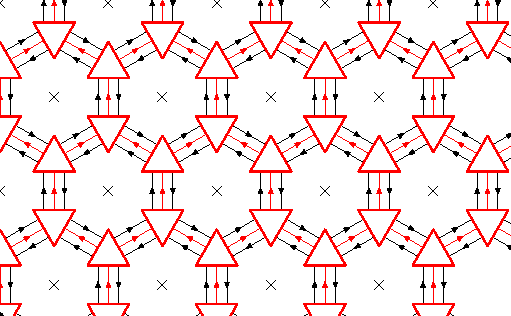
\includegraphics[width=0.6\textwidth]{images/temp/string-net-peps.pdf}
  \caption[弦网模型基态的 PEPS 张量网络表示]{弦网模型基态的 PEPS 张量网络表示。}
  \label{fig:string-net-peps}
\end{figure}

\section{奇异关联子}

\section{四面体对称性}

\section{MPO 对称性}

\section{例子}

\subsection{Fibonacci 模型}

\subsection{Ising 模型}
